\documentclass[11pt, oneside,a4paper]{article}
\usepackage[utf8]{inputenc}
\usepackage[english]{babel}
\usepackage{graphics}          %include graphics
\usepackage{float}             %better handling of tables, etc.

\usepackage{pythonhighlight}
\usepackage{tikz}
\usepackage{tikz-cd}


%mathematics
\usepackage{amssymb,amsmath, amsfonts, amsthm}
\usepackage{mathtools}
\usepackage{extarrows}

%setup for amsthm
\usepackage[intlimits]{esint}
\newtheorem{theorem}{Theorem}[section]
\newtheorem{lemma}[theorem]{Lemma}
\newtheorem{definition}[theorem]{Definition}
\newtheorem{corollary}[theorem]{Corollary}

\theoremstyle{definition}
\newtheorem{example}[theorem]{Example}
\newtheorem{counterexample}[theorem]{Counterexample}
\newtheorem{xca}[theorem]{Exercise}
\theoremstyle{remark}

\newtheorem{remark}[theorem]{Remark}

\usepackage{hyperref}
\usepackage[square, numbers]{natbib}
\bibliographystyle{abbrvnat}


%minor improvements to typesetting
\usepackage[activate={true,nocompatibility},final,tracking=true,kerning=true,spacing=true,factor=1100,stretch=10,shrink=10]{microtype}
\microtypecontext{spacing=nonfrench}
\microtypesetup{protrusion=true}

%adjust margins and headers
\usepackage{geometry,fancyhdr}
\geometry{a4paper,headheight=20pt, footskip=20pt, textheight=684pt, marginparwidth=10pt, textwidth=476pt}
\pagestyle{fancy}
\fancyhf{}
\lhead{Bachelor Thesis}
\rhead{Levi Moes}
\rfoot{\thepage}
\title{Bachelor Project \\
  Mordell's Theorem for Elliptic Curves with a point of Order 3}
\author{Levi Moes}

%commands
\newcommand{\legendre}[2]{\left( \frac{#1}{#2} \right)}
\newcommand{\emptyline}{\\ \hphantom{ } \\}
\DeclareMathOperator{\spa}{span}
\DeclareMathOperator{\re}{Re}
\DeclareMathOperator{\im}{Im}
\DeclareMathOperator{\Arg}{Arg}
\DeclareMathOperator{\id}{id}
\DeclareMathOperator{\lcm}{lcm}
\DeclareMathOperator{\tors}{tors}

\begin{document}
\maketitle

\begin{abstract}
  \noindent
  Tate-Silverman proves Mordell's theorem for curves with a point of order 2,
  we show this proof generalises to curves with a point of order 3.
\end{abstract}
\tableofcontents

\section{Introduction}
\label{sec:introduction}



\clearpage
\section{Cubic Polynomials}%
\label{sec:cubic_polynomials}
We expect the reader to be well familiar with methods of
finding roots of quadratic polynomials.
In particular we have the famous quadratic formula.

In this section we shall discuss some similar concepts of solving
cubic polynomials. In particular this thesis will be interested
in monic polynomials $f(x) = x^3 + ax^2 + bx + c$, where $a, b, c \in \mathbb{R}$.
Firstly, we will generalise the concept of the term $b^2 - 4ac$ in
the quadratic formula to such a cubic. Namely, we are looking
for a function that takes the coefficients of a polynomial
and outputs 0 if and only if it has a double root.

An obvious way to do this is to define
\[ \Delta(f) = \prod_{0 < i < j \leq 3}^{} (r_i - r_j)^2 \]
where $r_k$ is a root of $f(x)$. It can then be seen that $\Delta(f) = 0$
if and only if $r_i = r_j$ for some $i \neq j$, i.e.\ $f$ has
a double root.

We are able to simplify even more because of the following theorem
\begin{theorem}
  For any cubic $f(x) = ax^3 + bx^2 + cx + d$ the change of variables
  \begin{align*}
    x \mapsto t - \frac{b}{3a}
  \end{align*}
  yields a polynomial $f(t) = t^3 + pt + q$.
\end{theorem}
\begin{proof}
  This is a straightforward computation.
\end{proof}


\clearpage
\section{Projective Geometry}%
\label{sec:projective_geometry}

\clearpage
\section{Elliptic Curves}%
\label{sec:elliptic_curves}
The general notion of an elliptic curve shall be the centre of
focus for this thesis. One might define an Elliptic Curve as follows.
\begin{definition} \label{def:ellipticCurve}
  Let $f(x)$ be a 3rd degree monic polynomial having distinct roots.
  An Elliptic Curve is a curve
  \[ E: y^2 = f(x). \]
  If $K$ is a field, we denote for a given Elliptic Curve
  \[ E(K) := \left\{ (x,y) \in K \times K : y^2 = f(x) \right\} \cup \{\mathcal{O}\}, \]
  where $\mathcal{O}$ is the point at infinity.
\end{definition}
Since we are talking about an Elliptic \textit{Curve} it is tempting
to look at a case where $K$ allows us to draw a continuous line to
depict an Elliptic Curve.
\begin{example} \label{ex:curveExamplesContinuous}
  Take $K = \mathbb{R}$, $f(x) = x^3 + px^2 + 1$, where we let $r \in \left\{ -2,\dots, 3 \right\}$.
  This yields a sequence of Elliptic Curves $E_p$, we used
  python to depict these curves on $[-5, 5] \times [-5, 5]$.
  \begin{figure}[H]
    \centering
    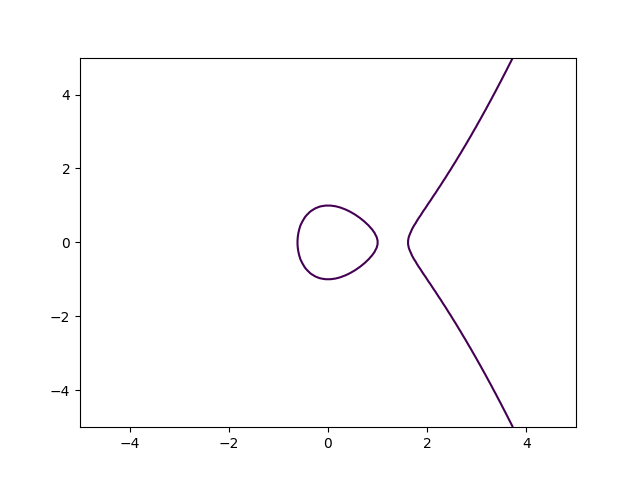
\includegraphics[width=0.3\linewidth]{ellipticCurves/example1p-2.png}
    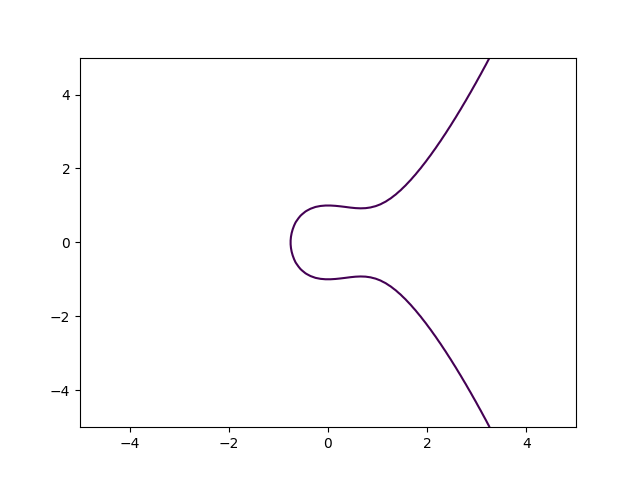
\includegraphics[width=0.3\linewidth]{ellipticCurves/example1p-1.png}
    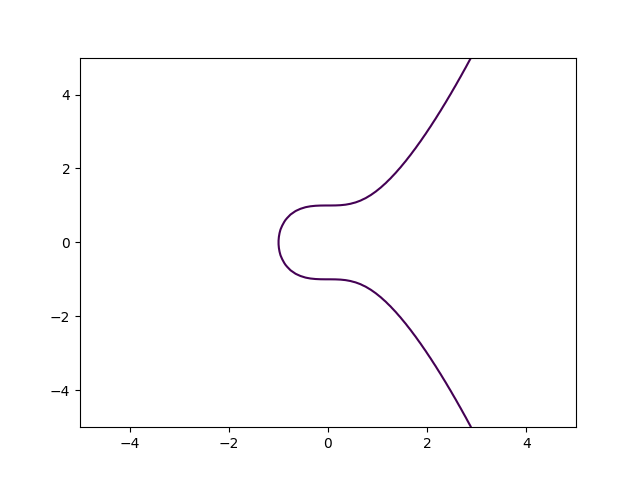
\includegraphics[width=0.3\linewidth]{ellipticCurves/example1p0.png}
    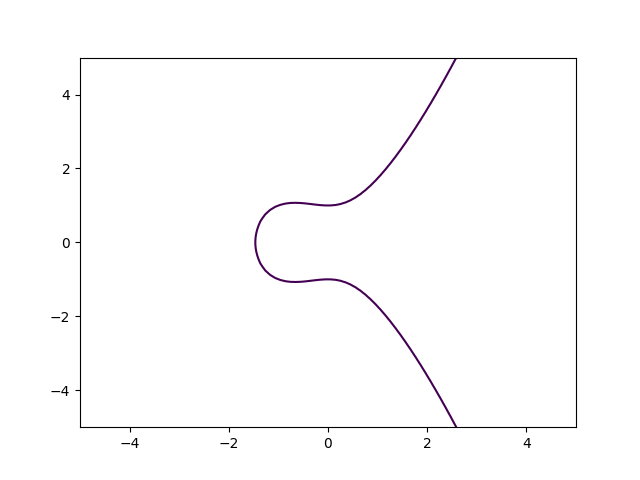
\includegraphics[width=0.3\linewidth]{ellipticCurves/example1p1.png}
    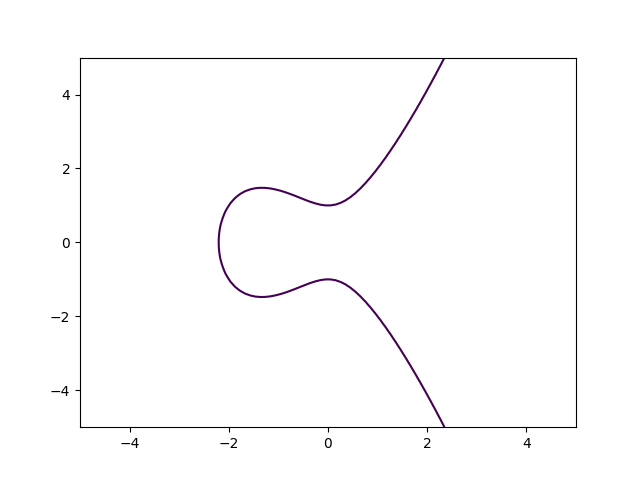
\includegraphics[width=0.3\linewidth]{ellipticCurves/example1p2.png}
    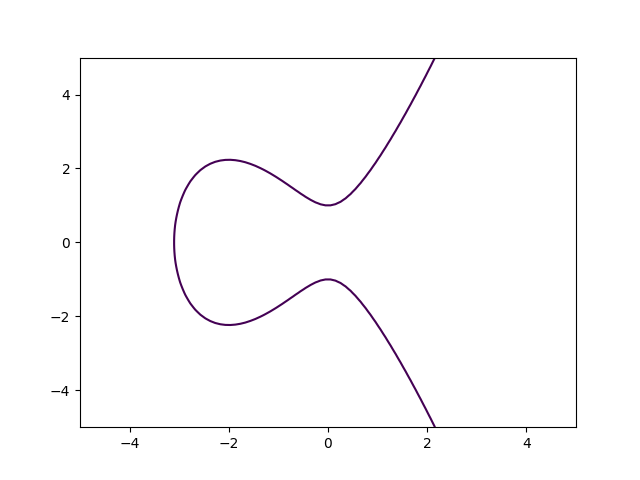
\includegraphics[width=0.3\linewidth]{ellipticCurves/example1p3.png}
    \caption{The curves $y^2 = x^3 + px^2 + 1$ for $p \in \{-2, \dots, 3\}$.}%
    \label{fig:curvesExamples}
  \end{figure}
\end{example}
It should be noted that an Elliptic Curve is not always a curve
in the Calculus sense, but may also consist of a series of seemingly
random points. As is illustrated in the following example.
\begin{example} \label{ex:curveExamplesFinite}
  Let $K = \mathbb{F}_{p}$, $p \equiv 3 \mod 4$ a prime and $f(x) = x^3 + nx$
  where $\gcd(n, p) = 1$.
  To find $E(\mathbb{F}_p)$ we wish to find when
  $x^3 + nx$ is a square modulo $p$.
  Note that $-1$ is not a square, since the Legendre Symbol equals
  \begin{align*}
    \left( \frac{-1}{p}  \right) = (-1)^{\frac{p-1}{2} } = (-1)^{\frac{3 + 4k - 1}{2} } = (-1)^{1 + 2 k} = -1.
  \end{align*}
  Fix some $a \in \mathbb{F}_p$ which is not a root of $f$,
  then
  \begin{align*}
    \legendre{a^3+na}{p}\legendre{(-a)^3+n(-a)}{p}
    = \legendre{a}{p}^2 \legendre{-1}{p}\legendre{a^3+na}{p}^2
    = -1.
  \end{align*}
  Hence precisely one of $f(a)$ and $f(-a)$ is a square.
  So for half of all residue classes $x$ we can find two points $(\sqrt{f(\pm x)},x)$ and
  $(-\sqrt{f(\pm x)}, x)$ on the curve. Hence including the point at infinity
  we have
  \begin{align*}
    \# E(\mathbb{F}_p) = p + 1.
  \end{align*}
  For instance when $p = 7$ we have
  \begin{align*}
    E(\mathbb{F}_p) = \left\{ \mathcal{O}, (0, 0), (3, 1), (4, 1), (3, 3), (4, 3), (2, 5), (5, 5) \right\}.
  \end{align*}
\end{example}
The main reason we are interested in Elliptic Curves is that $E(K)$ is an Abelian Group.
In the case that $K = \mathbb{Q}$ there is a geometric interpretation of what
this means, which uses only calculus.

\subsection{Elliptic Curves over the Rationals}
\label{sub:elliptic_curves_over_the_rationals}
We take $E: y^2 = f(x)$ to be an Elliptic Curve over $\mathbb{Q}$.
As an example of such a curve we take $f(x) = x^3 - 6x + 9$.
Say we take two points on this curve, say $(-3, 0)$ and $(1,2)$.
Then note we can draw a line through both of these points and it intersects
the curve at a 3rd point.
\begin{figure}[H]
  \centering
  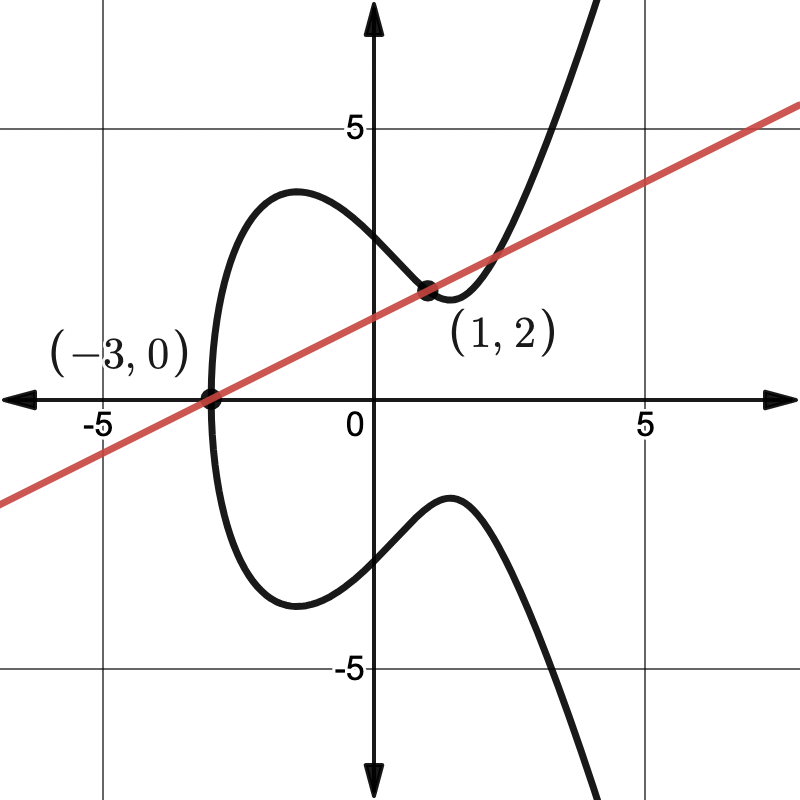
\includegraphics[width=0.5\linewidth]{ellipticCurves/ellipticCurveImage1.png}
  \caption{Two points on $y^2 = f(x)$ }%
  \label{fig:ellipticCurves/ellipticCurveImage1}
\end{figure}
In fact, barring a few exceptions, we can use this method to obtain
a 3rd point when we know two points on the curve.

When we have two distinct points $(x_1,y_1), (x_2,y_2) \in E(\mathbb{Q})$ we can use
calculus to find a line through both, namely the line
\begin{align*}
  y = \frac{y_2 - y_1}{x_2 - x_1} (x - x_1) + y_1.
\end{align*}
Note that this line does not intersect the curve in a 3rd point in $\mathbb{Q}$
when $y_1 = y_2$. Barring this case though, we find via a straightforward computation
that
\begin{equation} \label{eq:3rdPoint}
  x_3 = \left[ \frac{y_2 - y_1}{x_2 - x_1}  \right]^2 - (x_1 + x_2), \qquad y_3 = y_1 + \frac{y_2 - y_1}{x_2 - x_1} (x_3 - x_1)
\end{equation}
is also a point on this curve.

If the points are not distinct, then \cite[chapter 1.4]{silvermanRationalPoints}
describes how we can similarly use the tangent line, which also leads
to a point with coordinates in $\mathbb{Q}$.
\emptyline
At this point it is tempting to define a group law
by mapping $*: ((x_1,y_1), (x_2, y_2)) \mapsto (x_3, y_3)$. Sadly this
is not associative.

\begin{counterexample} \label{counterexample:notAssociative}
  Let $E: y^2 = f(x)$ as above over $\mathbb{Q}$.
  We find the line through $(-3, 0), (1,2)$ to be
  \begin{align*}
    y = \frac{x}{2} + \frac{3}{2}.
  \end{align*}
  and we solve
  \begin{align*}
    \left(\frac{x}{2} + \frac{3}{2}\right)^2 = x^3 - 6x + 9
  \end{align*}
  which has a solution $9/4$, giving a 3rd point $(9/4, 9/8 + 3/2)$,
  which we set $(-3, 0) * (1, 2)$.  Now similarly we compute $((-3, 0) * (1,2)) * (-1.414, 3.828) = (-0.727,3.602)$.

  On the other hand, we find
  $ (1,2) * (-1.414, 3.828) = (0.9879, 2.0092) $
  and thus so we find $(-3, 0) * (0.9879, 2.0092) = (2.266, 2.6531)$
\end{counterexample}

\subsubsection{The Group law}%
\label{ssub:the_group_law}
Luckily a small modification of $*$ does yield an associative operation,
namely when we take the 3rd point of intersection, and take its
antipode in the $y$ axis.
\begin{figure}[H]
  \centering
  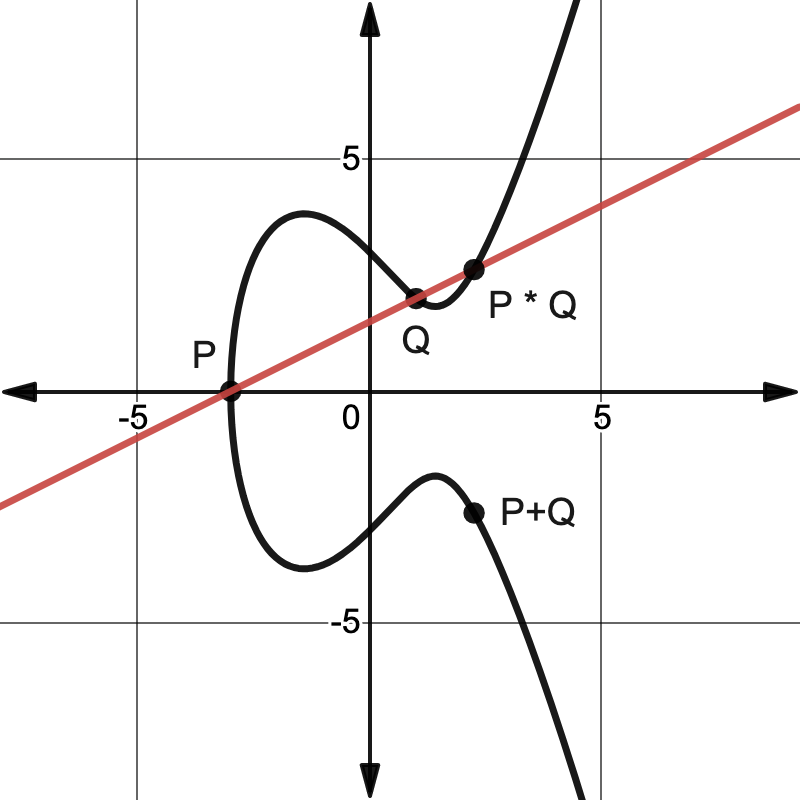
\includegraphics[width=0.5\linewidth]{ellipticCurves/ellipticCurveImage2.png}
  \caption{Depiction of the group law}%
  \label{fig:ellipticCurves/ellipticCurveImage2}
\end{figure}
This still leaves a number of edge cases.
For instance, when two points are antipodes
there is not going to be a 3rd point of intersection in $\mathbb{Q}^2$.
Luckily we have a point at infinity, which we will define
to be the sum of two antipodes.

After this motivation we introduce the following definition,
which is used by \cite[section 1.4]{silvermanRationalPoints}.
\begin{definition} \label{def:groupLaw}
  Let $P = (x_1, y_1), Q = (x_2, y_2)$ be points on an Elliptic curve $y^2 = x^3 - ax - b$, define an operation $+_E$ as follows.
  \begin{enumerate}
    \item If $P \neq Q$ and $x_1 = x_2$ then $P +_E Q = \mathcal{O}$.
    \item If $P = Q$ and $y_1 = 0$ then $P +_E Q = \mathcal{O}$
  \end{enumerate}
  If neither of these are the case we define $\lambda$ and $\nu$ as follows.
  \begin{enumerate}
    \item if $P \neq Q$ and $x_1 \neq x_2$
      then
      \[ \lambda = \frac{y_2 - y_1}{x_2 - x_1},\qquad \nu = \frac{y_1x_2 - y_2 x_1}{x_2 - x_1}.\]
    \item If $P = Q$ and $y_1 \neq 0$ then
      \[ \lambda = \frac{3x_1^2 + a}{2y_1},\qquad \nu = \frac{-x_1^3 + ax_1 + 2b}{2y_1} \]
  \end{enumerate}
  then
  \[ P +_E Q = (\lambda^2 - x_1 - x_2, -\lambda^3 + \lambda (x_1 + x_2) - \nu). \]
  When it is clear from context what the curve is, we will write $+$ instead of $+_E$.
\end{definition}
So we have a set, together with a binary operation. This
motivates the following theorem.
\begin{theorem}
  Let $E: y^2 = f(x)$ be an elliptic curve. Then
  $(E(\mathbb{Q}), +_E, \mathcal{O})$ is an Abelian Group.
\end{theorem}
\begin{proof}
  By construction, we have that $+_E: E(\mathbb{Q}) \times E(\mathbb{Q}) \to E(\mathbb{Q})$
  is well defined. Namely, it is clear from equation \ref{eq:3rdPoint}
  that when $P, Q \in E(\mathbb{Q})$, then also $P * Q \in E(\mathbb{Q})$.
  Consequently, the projection in the $y-axis$ is also in $E(\mathbb{Q})$.

  Moreover, if we have a line $y = ax + b$ through $P, Q \in E(\mathbb{Q})$, then
  this yields an equality
  \begin{align*}
    \left(\frac{y_2 - y_1}{x_2 - x_1} (x - x_1) + y_1\right)^2 = x^3 + px^2 + qx + r
  \end{align*}
  Which yields a root finding problem $\tilde{f}(x) = 0$.
  We know that we can factor $\tilde{f}(x) = (x - x_1)(x - x_2)(x - A)$,
  for some $A$. We argue $A$ must be rational, since if $A \notin \mathbb{Q}$,
  then we would have
  \begin{align*}
    \tilde{f}(x) = -A x_1 x_2 + A x_1 x + A x_2 x - A x^2 + x_1 x_2 x - x_1 x^2 - x_2 x^2 + x^3
  \end{align*}
  not having rational coefficients. But clearly $\tilde{f}$ must have rational coefficients,
  we conclude $A$ is the $x$ coordinate of a 3rd point of intersection, and moreover
  there cannot be any more factors, so there are precisely 3 points of intersection.
  So indeed $+_E$ is well-defined.

  It should also be clear that $+_E$ is commutative, since $P +_E Q$ and $Q +_E P$ would
  yield the same 3rd point of intersection.

  Inverses are also straightforward: we think of $\mathcal{O}$ of sitting at infinity,
  so the line through a point and its antipode (which may be the point itself if we are
  talking about points like $(-3, 0)$ as in \ref{fig:ellipticCurves/ellipticCurveImage1})
  will only intersect at infinity.

  The proof of $+_E$ being associative can be found in \cite[section 2.4]{washingtonElliptic}
\end{proof}
We shall from now on just denote $E(\mathbb{Q})$ to indicate this group.
\begin{example}
  The curve $E: y^2 = x^3 - 6x^2 -9x + 1$ over $\mathbb{Q}$ is
  finitely generated.
  Using SageMath we found
  \begin{python}
sage: E = EllipticCurve([0,-6,0,-9,1]); E
Elliptic Curve defined by y^2 = x^3 - 6*x^2 - 9*x + 1 over Rational Field
sage: E.gens()
[(0 : 1 : 1), (240 : 3671 : 1)]
sage: E.rank()
2
  \end{python}
  Hence using the structure theorem we find there is some Abelian group $A$
  such that
  \begin{align*}
    E(\mathbb{Q}) \simeq \mathbb{Z}^2 \times A
  \end{align*}

\end{example}

\subsection{Elliptic Curves over an Arbitrary Field}%
\label{sub:elliptic_curves_over_an_arbitrary_field}
In an arbitrary field we can define $+$ analogously to definition \ref{def:groupLaw}.
And again we have
\begin{theorem}
  Let $K$ be a field, and $E: y^2 = f(x)$ an elliptic curve.
  Then $(E(K), +_E, \mathcal{O})$ is an Abelian Group.
\end{theorem}
This yields the following
\begin{example} \label{ex:curveOfPplus1}
  Let $p$ be a prime and $E: y^2 = f(x)$ an elliptic curve.
  For any finite field $\mathbb{F}_{p^n}$ we surely have
  $E(\mathbb{F}_{p^n})$ is finite. So by the structure theorem
  \cite[theorem 2.8]{sergeLangAlgebra}
  there exist finitely many $a_i \in \mathbb{N}_0$
  such that
  \begin{align*}
    E(\mathbb{F}_{p^{n}}) \simeq \mathbb{Z}/a_0\mathbb{Z} \times \dots \times \mathbb{Z}/a_{k}\mathbb{Z}.
  \end{align*}
  In example \ref{ex:curveExamplesFinite} we found that for
  $p \equiv 3 \mod 4$ a curve $E: y^2 = x^3 + nx$ has $\# E(\mathbb{F}_p) = p + 1$.

  When $p = 43$ we have $\#E(\mathbb{F}_{43}) = 44 = 2^2 \cdot 11$,
  hence the only two Abelian groups of this order are
  $\mathbb{Z}/11\mathbb{Z} \times \mathbb{Z}/4\mathbb{Z}$ and
  $\mathbb{Z}/11\mathbb{Z} \times \mathbb{Z}/2\mathbb{Z} \times \mathbb{Z}/2\mathbb{Z}$.
  It can be verified that $(42, 27)$ is a point of order 4, so
  \begin{align*}
    E(\mathbb{F}_{43}) \simeq \mathbb{Z}/11\mathbb{Z} \times \mathbb{Z}/4\mathbb{Z} \simeq \mathbb{Z}/44\mathbb{Z}.
  \end{align*}
  Numerically, it appears that when $n$ is a square these groups
  are always cyclic.
\end{example}
There is a well-known class of primes which have some nice behaviour over
these curves
\begin{example} \label{ex:mersenneCurve}
  Let $E: y^2 = f(x)$ over $\mathbb{F}_{p}$ be as in example \ref{ex:curveOfPplus1}.
  There is the famous class of Mersenne Primes, which are primes of
  the form $2^p - 1$, where $p$ is a prime. An efficient
  algorithm exists to determine the primality of these numbers
  \cite{bruceLLTest}
\end{example}

\subsection{Isogenies}%
\label{sub:isogenies}
Since we know that an Elliptic Curve $E: y^2 = f(x)$ over a
field $K$ has an associated group $E(K)$, it is natural
to speak about group homomorphisms between these groups.
This leads us to the following definition.
\begin{definition} \label{def:isogeny}
  Let $E_1, E_2$ be Elliptic Curves over a field $K$.
  An isogeny $\varphi: E_1(K) \to E_2(K)$ is a rational function
  that is also a group homomorphism.
\end{definition}
The astute reader might notice that this definition is
over-engineered, as one can prove that any rational function
$\varphi: E_1(K) \to E_2(K)$ satisfying $\varphi: \mathcal{O} \mapsto \mathcal{O}$
would automatically be a group homomorphism. And this is indeed what
Silverman proves \cite[Theorem III.4.8]{silvermanRationalPoints}
the following theorem.
\begin{theorem} \label{thm:rationalMapsAreIsogeny}
  Let $E_1, E_2$ be Elliptic Curves over a field $K$
  and $\varphi: E_1(K) \to E_2(K)$ be rational maps
  such that $\varphi(\mathcal{O}) = \mathcal{O}$,
  then $\varphi$ is a group homomorphism.
\end{theorem}
Below we shall go into some examples
that shall come in useful later.
\begin{example} \label{ex:multiplicationIsogeny}
  Fix some $n \in \mathbb{N}$ then $[n]: P \mapsto nP$ is an isogeny, since
  it is clearly a rational function, and it is also a homomorphism
  of groups as by definition $n \mathcal{O} = \mathcal{O}$. And since
  the group of rational points on an elliptic curve is abelian
  \[ nA + nB = A + \dots A + B + \dots B = A + B + \dots + A + B = n(A+B). \]
\end{example}
The following example is the subject of \cite[chapter 2.2]{moniqueThesis}
\begin{example} \label{eq:dualIsogenies}
  Let $A, B \in \mathbb{Q}$ and $\bar{A} = -27A, \bar{B} = 4A + 27B$
  \begin{align*}
    E: y^2 = x^3 + A(x - B)^2, \qquad \bar{E} \eta^2 = \xi^3 + \bar{A} (\xi - \bar{B})^2
  \end{align*}
  be Elliptic Curves, we define the map
  \[ \Phi_{X, Y}: (x, y) \mapsto (\xi, \eta), \]
  where
  \begin{align*}
    \xi &=  \frac{9}{x^2} \left( 2y^2 + 2XY^2 - x^3 - \frac{2}{3} X x^2  \right), \\
    \eta &= \frac{27y}{x^3} \left( -4XYx + 8XY^2 - x^3 \right).
  \end{align*}
  If we define $\Phi_{X, Y}: \mathcal{O} \mapsto \mathcal{O}$ then by
  theorem \ref{thm:rationalMapsAreIsogeny} it follows
  that $\Phi_{X, Y}$ is an isogeny.
  If we apply the map $\Phi_{\bar{A}, \bar{B}} \circ \Phi_{A, B}$
  we obtain the curve
  \begin{align*}
    C: y^2 = x^3 + 3^{6}A(x - 3^6 B)^2.
  \end{align*}
  The change of coordinates
  \begin{align*}
    (x, y) \mapsto (3^6 x, 3^9 y)
  \end{align*}
  gives
  \begin{align*}
    3^{18}y = 3^{18}x^2 + 3^{18}A(x - B)^2
  \end{align*}
  which is the equation of $E$ multiplied by $3^{18}$.
  In conclusion the following diagram commutes
  \begin{equation*}
  \begin{tikzcd}
    E(\mathbb{Q}) \ar[rr, bend left, "\begin{bmatrix}3\end{bmatrix}"] \ar[r, "\Phi_{A, B}"] & \bar{E}(\mathbb{Q}) \ar[r, "\Phi_{\bar{A}, \bar{B}}"] & C(\mathbb{Q})
  \end{tikzcd}
  \end{equation*}

\end{example}


\clearpage
\section{Points of Finite Order}%
\label{sec:points_of_finite_order}
We shall introduce the concept of torsion in the
context of Abelian groups, after this we will
use this to prove properties of the torsion subgroup
of the rational points on an elliptic curve.
\begin{definition}
  Let $A$ be an Abelian group. A point of finite order
  is called a torsion point. We denote the set of all
  torsion points in $A$ as $A_{\tors}$.
\end{definition}
\begin{theorem}
  $A_{\tors}$ is a subgroup of $A$.
\end{theorem}
\begin{proof}
  Let $(A, e, *)$ be an Abelian group and $H = \left\{ x \in A : |x| < \infty \right\}$,
  then $H \leq A$ since clearly $e \in H$ and when $x,y \in H$ then
  $|xy^{-1}| = \lcm(|x|, |y^{-1}|) = \lcm(|x|, |y|) < \infty$.
\end{proof}
\begin{definition}
  Let $(A, e, *)$ be an Abelian group, define
  \[ A[n] := \left\{ x \in A : x^n = e \right\}  \]
\end{definition}
\begin{theorem}
  $A[n]$ is a subgroup of $A_{\tors}$
\end{theorem}
\begin{proof}
  Note that $A[n]$ is precisely the kernel of $f: x \mapsto x^n$,
  therefore it must be a subgroup, since clearly $e \in \ker f$ and
  moreover $x, y \in \ker f$ means $f(xy^{-1}) = f(x) f(y^{-1}) = f(x) f(y)^{-1} = e$.
\end{proof}
\begin{example} \label{ex:torsionFinite}
  If $K$ is finite then $E(K) = E(K)_{\tors}$ follows by Lagrange's Theorem.
\end{example}
\begin{example} \label{ex:torsionInfinite}
  A point of order 2 must have a vertical tangent line.
  Consider the curve $y^2 = x^3 + 6x^2 + 5x$ over $\mathbb{Q}$,
  the points with such a tangent line are depicted in figure \ref{fig:pointsOfFiniteOrder/examplePointsOfOrder2}.
  \begin{figure}[H]
    \centering
    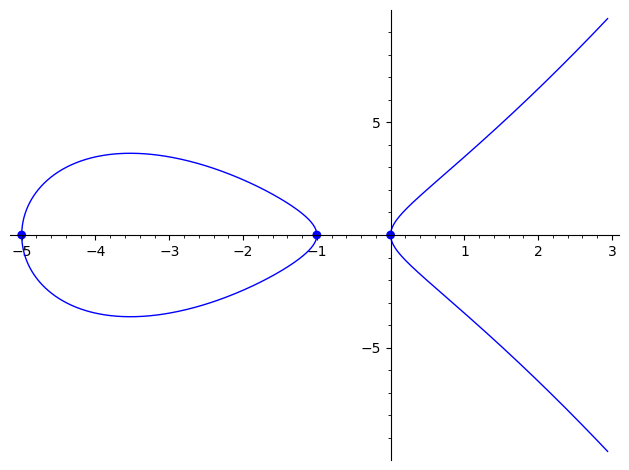
\includegraphics[width=0.3\linewidth]{pointsOfFiniteOrder/examplePointsOfOrder2.png}
    \caption{Points of order 2 on $y^2 = x^3+6x^2 + 5x$ over $\mathbb{Q}$ }%
    \label{fig:pointsOfFiniteOrder/examplePointsOfOrder2}
  \end{figure}
  \noindent
  There are three such points, so we have
  \[ E(\mathbb{Q})[2] = \left\{ \mathcal{O}, (-5 , 0), (-1 , 0 ), (0 , 0) \right\}. \]
  In particular this tells us $E(\mathbb{Q})[2] \simeq \mathbb{Z}/2\mathbb{Z} \times \mathbb{Z}/2\mathbb{Z}$,
  since this is a group of 4 elements and
  all points besides the identity have order 2.
\end{example}
\subsection{The Nagell-Lutz Theorem}%
\label{sub:the_nagell_lutz_theorem}
\begin{theorem} \label{thm:nagellLutz}
  Let $E: y^2 = f(x)$ be an Elliptic Curve over $\mathbb{Q}$.
  All torsion points of $E(\mathbb{Q})$ have integer coordinates.
  Moreover if $(x,y) \in E(\mathbb{Q})_{\tors}$
  and $y = 0$ then $P$ has order 2, else $y|D$,
  the discriminant of $f$.
\end{theorem}

\subsection{Points of Order 2}%
\label{sub:points_of_order_2}

\subsection{Points of Order 3}%
\label{sub:points_of_order_3}
A point $P$ having order $3$ may be phrased as $2P = -P$,
so this means that the $x$ coordinates of $-P$ and $2P$ must be the same.
For an elliptic curve $y^2 = x^3 + ax^2 + bx + c$
one can find that the $x$ coordinate of $2P$ is given by
\begin{equation} \label{eq:xcord2p}
  F(x) = \frac{x^4 -2bx^2 - 8xcx + b^2 - 4ac}{4x^3+4ax^2 + 4bx+4c}
\end{equation}
so a point of order 3 is a fixed point $F(x) = x$, so
\begin{align*}
  F(x) = x &\iff \frac{x^4 -2bx^2 -8cx + b^2 - 4ac}{4x^3+4ax^2 + 4bx+4c} = x \\
           &\iff x^4 -2bx^2 -8xcx + b^2 - 4ac = 4x^4+4ax^3 + 4bx^2+4cx \\
           &\iff \underbrace{3x^{4} + 4ax^3 + 6bx^2 + 12 cx + 4ac - b^2}_{\psi_3} = 0.
\end{align*}
Silverman notes that $\psi_3 = 2f(x)f''(x) - f'(x)^2$ \cite[section 2.1]{silvermanRationalPoints}.
So points of order 3 are roots of this polynomial.
\begin{theorem}
  Let $E: y^2 = f(x)$ be an Elliptic Curve.
  Then $\mathcal{O} \neq P \in E(\mathbb{Q})$ has order 3
  if and only if it is a point of infliction.
\end{theorem}
This result is an exercise in the book of Tate and Silverman
\cite[Exercise 2.2]{silvermanRationalPoints}.
\begin{proof}
  We first find the second derivative, using the chain rule
  \begin{align*}
    \frac{\mathrm{d}^2y}{\mathrm{d}x^2} = \frac{\mathrm{d}^2 \sqrt{y^2} }{\mathrm{d}^2 x}
    = \frac{\mathrm{d}}{\mathrm{d}x} \left[ \frac{\mathrm{d}^2 \sqrt{y^2} }{\mathrm{d}y^2} \frac{\mathrm{d}y^2}{\mathrm{d}x}   \right]
    = \frac{\mathrm{d}}{\mathrm{d}x} \left[ \frac{1}{2 \sqrt{y^2}} f'(x)   \right]
    = \left[\frac{\mathrm{d}}{\mathrm{d}x}\frac{1}{2y} \right] f'(x)
    + \frac{1}{2y} f''(x).
  \end{align*}
  Note that
  \begin{align*}
    \frac{\mathrm{d}}{\mathrm{d}x} \frac{1}{2y} = \frac{\mathrm{d}}{\mathrm{d}y^2} \frac{1}{2y} \frac{\mathrm{d}y^2}{\mathrm{d}x}
    = -\frac{1}{4 y^3} f'(x)
  \end{align*}
  putting this all together we obtain
  \begin{align*}
    \frac{\mathrm{d}^2y}{\mathrm{d}x^2} = -\frac{1}{4y^3} f'(x)^2 + \frac{1}{2y} f''(x)
    = \frac{2y^2}{4y^3} f''(x) - \frac{1}{4y^3}f'(x)^2
    = \frac{2f(x)f''(x) - f'(x)^2}{4yf(x)}
    = \frac{\psi_3(x)}{4y f(x)},
  \end{align*}
  since $y^2 = f(x)$.
  Since a point $(x_0, y_0)$ of order 3 has $\psi_3(x_0) = 0$,
  it follows that $(x_0, y_0)$ is an infliction point
  if and only if $(x_0, y_0)$ has order 3.
\end{proof}
So finding a point of order 3 reduces to finding the roots
of the quartic polynomial $\psi_3$.
From the fundamental theorem of algebra, it then follows
that for every elliptic curve there is a point of order
3 in $E(\mathbb{C})$, but we are interested in rational
points. We shall prove several lemmas which lead up to a
result about points of order 3.
\begin{lemma}
  $\psi_3$ has distinct roots in $\mathbb{C}$.
\end{lemma}
This similar to a result in the book by Tate and Silverman \cite[theorem 2.1]{silvermanRationalPoints}
\begin{proof}
  Recall $\psi_3(x) = 2 f(x)f''(x) - f'(x)^2$, so via the product
  rule
  \[ \psi_3' = 2 \left[ f'f'' + f'''f \right] - 2f'f'' \]
  but $f$ is monic of order 3, so $f''' = 6$, so
  $\psi_3' = 12f$. Since $f$ cannot share any roots with $f'$
  it follows that $\psi_3$ and $\psi_3'$ do not share any roots.
  In conclusion, $\psi_3$ has distinct complex roots.
\end{proof}
\begin{lemma}
  $\psi_3$ has precisely 2 real roots.
\end{lemma}
This is again an exercise in Tate-Silverman \cite[Exercise 2.2b]{silvermanRationalPoints}.
\begin{proof}
  We compute $f''(x) = 6x + 2a$, this has a root $x = -a/3$.
  Since $f'(x) = 3x^2 + 2ax + b$ we find $f'(-a/3) = -a^2/3 -2a^2/3 + b = b - a^2$.
  So
  \[ \psi_3(-a/3) = -(b-a^2)^2 < 0. \]
  But surely the term $3x^4$ is going to be much larger than the lower
  order terms, so at some point $0 \neq x_0 > -a/3$ it is the case that $\psi_3(x_0) > 0$ and $\psi_3(-x_0) > 0$ .
  So by the intermediate value theorem \cite[theorem 4.35]{sutherlandMTS}
  we get the existence of two real roots.

  The coefficients of $\psi_3$ are all real, so we cannot have
  precisely 3 real roots, as then we could find $x_4 \notin \mathbb{R}$
  and so
  \[ \psi_3 = \prod_{i=1}^{4} (x - x_i) = x \prod_{i=1}^{3}(x-x_i) - x_4 \prod_{i=1}^{3} (x - x_i) \notin \mathbb{R}[x].  \]
  So we can only have 2 or 4 real roots.

  Suppose we have $x_1 < x_2 < x_3 < x_4$ real roots, where
  $x_1$ and $x_4$ are the roots we proved exist.
  Then at two points between $x_1$ and $x_4$: $\psi_3' = 12f$ must change sign.
  It follows $f''(x_2) > -a/3$. By the same argument applied to $x_3$ and
  $x_4$ we find $x_3 < -a/3$ so $x_2 > x_3$ which contradicts our ordering.
  Rearranging this argument for all possible orderings of the roots
  can be done similarly.
\end{proof}

\begin{example}
  When $a = 0$ and $c = 0$
  we get an elliptic curve $y^2 = x^3 + bx$
  our $\psi_3$ can be factored easily, since then
  the famous quadratic formula can be used to find
  \begin{align*}
    3x^4 + 6bx^2 - b^2 = 0 &\iff
    x^2 = -b \pm 2/3 \sqrt{3} b
    \iff
    x = \pm \sqrt{-b \pm 2/3 \sqrt{3} b}
  \end{align*}
  so such an elliptic curve never has
  a rational point of order 3 because this $x$ is never rational unless
  $b = 0$, which is a singular curve and hence not elliptic.
\end{example}
\begin{example}
  Consider the curve $E: y^2 = x^3 + x^2 + 2x + 1$ over $\mathbb{Q}$.
  This gives polynomial
  \begin{align*}
    \psi_3 = 3x^4 + 4x^3 + 12x^2 + 12x
  \end{align*}
  which has a rational root $x = 0$.
  Hence the points $(0, \pm 1)$ are of order 3, and moreover these
  are the only points of order 3. Giving us $E(\mathbb{Q})[3] \simeq \mathbb{Z}/3\mathbb{Z}$.
  \begin{figure}[H]
    \centering
    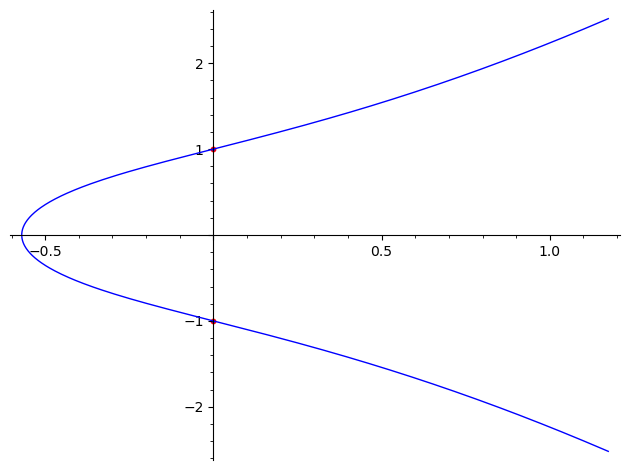
\includegraphics[width=0.4\linewidth]{pointsOfFiniteOrder/examplePointsOrder3.png}
    \caption{Points of order 3 on $y^2 = x^3 + x^2 + 2x + 1$ }%
    \label{fig:pointsOfFiniteOrder/examplePointsOrder3}
  \end{figure}
\end{example}
For some more general Elliptic Curves we can find if a point of order 3 exists as follows.
\begin{corollary}
  Suppose the coefficients of our Elliptic Curve are integers: $a, b, c \in \mathbb{Z}$.
  Then any point of order 3 has $x$-coordinate dividing $4ac - b^2$.
\end{corollary}
\begin{proof}
  From the rational root theorem \cite[Section 9.4]{dummiteAndFooteAbstractAlgebra}
  any rational root of $\psi_3$ has the form $x = p/q$ where $\gcd(p, q) = 1$, $p | 4ac - b^2$ and $q|3$,
  moreover we know from theorem \ref{thm:nagellLutz}
  that $p/q \in \mathbb{Z}$, so $q | p$. If $q = 3$ then $\gcd(p, q) = 3$
  which is not in lowest terms, so we have $q = 1$.
  For any rational solution $x$ we have $x|4ac - b^2$.
\end{proof}
\begin{example}
  For the Elliptic Curve
  $y^2 = x^3 + 3x^2 + 3x + 2$ we have
  any rational solution $x$ has
  $x|15$.
  By trying all divisors of $15$ we find $\psi_3(-1) = 0$ and
  hence we conclude $(0,-1)$ is a point of order 3.
\end{example}
\begin{example}
  The Elliptic Curve $y^2 = x^3 -9x + 9$
  has $b^2 - 4ac = -81$, which has divisors
  $\pm 1, \pm 3, \pm 9, \pm 81$.
  So by trial and error on
  \begin{align*}
    \psi_3 = 3x^4 - 54x^2 + 108x - 81
  \end{align*}
  we find that $\psi(3) = 0$.
  Hence $(3, \pm 3)$ are points of order 3.
\end{example}
\begin{example}
  The curve $y^2 = x^3 + 1$ is quite interesting.
  Since it contains both a point of order 2 and a point of order 3,
  clearly $-1$ is a root of $x^3 + 1$, which corresponds to a point (0, -1) of order 2,
  while $0$ is a root of $\psi_3$ so $(\pm 1, 0)$ are points of order 3.
  So we multiply a point of order 2 with a point of order 3 to give us a point of order 6,
  namely the point $(3, 2)$ has order 6.
\end{example}


\clearpage
\section{Mordell's Theorem}%
\label{sec:mordell_s_theorem}
\begin{theorem}
  For any Elliptic Curve $E: y^2 = f(x)$ the group $E(\mathbb{Q})$ is finitely
  generated.
\end{theorem}
Which requires results from cohomology which are beyond the
scope of this thesis \cite[Section VIII]{silvermanArithmetic} .
We shall prove the weaker version
\begin{theorem} \label{thm:mordell}
  Let $E: y^2 = f(x)$ be an Elliptic Curve. If
  $E(\mathbb{Q})$ contains a point of order 3, then
  $E(\mathbb{Q})$ is finitely generated.
\end{theorem}


\clearpage
\section{The 3-Descent Theorem}%
\label{sec:the_3_descent_theorem}
Our main tool for proving Mordell's Theorem for such curves
is the $3$-descent theorem.
\begin{theorem} \label{thm:3descent}
  Let $A$ be an Abelian group.
  Suppose there exists a function
  $h: A \to \mathbb{R}$
  such that for all $P \in A$
  \begin{enumerate}
    \item Let $Q \in A$ there
      is $C_1(A, Q) \in \mathbb{R}$
      such that
      \begin{equation} \label{eq:boundHeight}
        h(P + Q) \leq 2h(P) + C_1(A, Q).
      \end{equation}
    \item There is $C_2(A)$ such that
      \begin{equation} \label{eq:boundMultipleHeight}
        h(3P) \geq 9 h(P) - C_2(A).
      \end{equation}
    \item For every constant $C_3$
      the set
      \begin{equation} \label{eq:finitePoints}
        \left\{ Q \in A : h(Q) \leq C_3 \right\}
      \end{equation}
      is finite.
    \item The quotient group
      \begin{equation} \label{eq:quotient}
        A/3A
      \end{equation}
      is finite.
  \end{enumerate}
  Then $A$ is finitely generated.
\end{theorem}
We call such a function a \textit{height function}.
This theorem is the case $m = 3$ of the general descent theorem
\cite[theorem 3.1]{silvermanArithmetic}.
After we have this tool, proving theorem \ref{thm:mordell}
reduces to proving each of the conditions.
The proof of this mirrors the one given
by Silverman for the general descent theorem.
\begin{proof}
  Since we assume $A/3A$ is finite, take representatives
  $Q_1, \dots, Q_n \in A$ as representatives of the conjugacy classes.
  In addition, take arbitrary $P \in A$.
  Our goal will be to show $P - h(Q)$
  where $Q$ is some linear combination of
  the $Q_1, \dots, Q_n$ is arbitrarily small,
  allowing us to conclude the
  $Q_1,\dots, Q_n$ together
  with the points with smaller height
  are a generating set for $E(\mathbb{Q})$.

  We write $P = 3P_1 + Q_{i_1}$ for some $1 \leq i_1 \leq r$.
  Repeat this for $P_1$ to obtain a sequence
  \begin{align*}
    P &= 3P_1 + Q_{i_1}, \\
    P_1 &= 3P_2 + Q_{i_2}, \\
    \vdots \\
    P_{r-1} &= 3P_{r} + Q_{i_r}.
  \end{align*}
  this gives that for any index $j$:
  \begin{align*}
    h(P_j) &\leq \frac{1}{3^2}(h(3P_j) + C_2) \\
           &= \frac{1}{3^2} \left( h(P_{j-1} - Q_{i_j}) + C_2 \right) \\
           &\leq \frac{1}{3^2} ( 2h(P_{j-1} + \underbrace{\max \left\{ -Q_1, \dots, -Q_n \right\}}_{C_1'} + C_2) )
  \end{align*}
  Now we apply this inequality repeatedly,
  and note a geometric series
  \begin{align*}
    h(P_r) &\leq \left( \frac{2}{3^2}  \right)^{r} h(P) + \left[ \frac{1}{3^2} + \frac{2}{(3^2)^2} + \dots + \frac{2^{r-1}}{(3^2)^{r}}(C_1'+C_2)   \right] \\
         &< \left( \frac{2}{3^2}  \right)^{r} h(P) + \frac{C_1' + C_2}{3^2 - 2}  \\
         &\leq \frac{1}{2^r} h(p) + \frac{1}{2} (C_1' + C_2)
  \end{align*}
  so for sufficiently large $r$
  \begin{align*}
    h(P_r) \leq 1 + \frac{1}{2} (C_1' + C_2).
  \end{align*}
  And because $P$ is a linear combination of $P_r$ and the $Q_i$ we have
  \begin{align*}
    P = 3^{r} P_r + \sum_{j=1}^{r} 3^{j-1} Q_{i_j}
  \end{align*}
  so any $P \in A$ can be written as a linear combination of
  \begin{align*}
    \left\{ Q_1, \dots Q_r \right\} \cup \left\{ Q \in A : h(Q) \leq 1 + 1/2(C_1' + C_2) :  \right\}
  \end{align*}
  which is assumed to be finite.
\end{proof}


\clearpage
\section{Finding a Height Function}%
\label{sec:finding_a_height_function}
The remainder of this project will be about finding a height function
suitable for $E(\mathbb{Q})$, and then proving each of the properties
in theorem \ref{thm:3descent}.

We will first discuss a few examples so as to motivate an intuition behind
a height function.
\begin{example}
  In the case that $A = \mathbb{Q}$ we can define a function
  $h_{\mathbb{Q}}: \mathbb{Q} \to \mathbb{R}$
  \begin{equation} \label{eq:rationalHeight}
    h_{\mathbb{Q}}: p/q \mapsto \max \left\{ |p|, |q| \right\}
  \end{equation}
  and while it is known $\mathbb{Q}$ is not finitely generated
  as a group, we can still prove one of the properties from the
  3-descent theorem holds.
  Namely, we know that for fixed $m \in \mathbb{R}$ there
  are only finitely many rational numbers with height bounded
  by $m$. If $h(p/q) \leq m$ then both $p, q \leq m$,
  for which there are only finitely many possibilities.
\end{example}
\begin{definition} \label{def:ellipticHeight}
  (heights on Elliptic Curves)
  If $E: y^2 = f(x)$ is an Elliptic Curve over $\mathbb{Q}$, then
  we define the height of a point $P = (x,y)$ as
  $h(P) = h_{\mathbb{Q}}(x)$, where $h_{\mathbb{Q}}$ is
  as in equation \ref{eq:rationalHeight}.
\end{definition}
The remainder of this section shall be dedicated to proving
this notion of height satisfies theorem \ref{thm:3descent}.

\subsection{Bound on Height}%
\label{sub:bound_on_height}
Here we prove the first property of the 3-descent theorem, namely
\begin{lemma}
  Let $E: y^2 = f(x)$ be an Elliptic Curve.
  Then if $P \in E(\mathbb{Q})$ then for
  every $Q \in E(\mathbb{Q})$ there
  is an integer $C_1$ such that
  \begin{equation} \label{eq:boundOnHeightOfCurve}
    h(P + Q) \leq 2 h(P) + C_1.
  \end{equation}
\end{lemma}
This is found in \cite[section 3.2]{silvermanRationalPoints}.
\begin{proof}
  If $Q = \mathcal{O}$ then this
  is trivial.
  Suppose $Q \neq \mathcal{O}$,
  we prove that for all $P$ except
  for $ P \in \left\{ -Q, Q, \mathcal{O} \right\}$ there is
  $\tilde{C}_1$ such that \ref{eq:boundOnHeightOfCurve} holds.
  Then set $C_1 = \max\{h(-Q), h(Q), h(\mathcal{O}), \tilde{C}_1\}$.
\end{proof}


\clearpage
\section{The Quotient Group is Finite}%
\label{sec:the_quotient_group_is_finite}
Throughout this section it shall be well understood that
we are talking about an Elliptic Curve $C: y^2 = f(x)$
over $\mathbb{Q}$ such that $C(\mathbb{Q})$ has a point of order 3.
We shall moreover be using shorthand
\begin{equation*}
  \Gamma := C(\mathbb{Q})
\end{equation*}
This section shall be dedicated to proving the final part of
theorem \ref{thm:3descent}, that is
\begin{theorem} \label{thm:finiteIndex}
  The index $[\Gamma: 3\Gamma]$ is finite.
\end{theorem}
The sketch of our proof will be to define two classes
of curves $E: y^2 = g(\xi)$ and $\bar{E}: y^2 = h(x)$
and define two isogenies $\phi: E(\mathbb{Q}) \to \bar{E}(\mathbb{Q})$
along with $\bar{\phi}: \bar{E}(\mathbb{Q}) \to E(\mathbb{Q})$
such that $\phi \circ \varphi = P \mapsto 3P$.
This gives us an exact sequence
\begin{equation*}
\begin{tikzcd}
  0 \ar[r] & \bar{\phi}\bar{E}/3E \ar[r] & E/3E \ar[r] & E/\bar{\phi}\bar{E} \ar[r] & 0
\end{tikzcd}
\end{equation*}
We find an isomorphism
$f: \bar{\phi}\bar{E}/3E \to \mathbb{Q}(\sqrt{-3})^\times/(\mathbb{Q}(\sqrt{-3})^\times)^3$
and a homomorphism $g: E(\mathbb{Q}) \to \mathbb{Q}^\times/(\mathbb{Q}^\times)^3$ with kernel
$\bar{\phi}\bar{E}(\mathbb{Q})$ and show their images are finite.
Which means $E/3E$ must be finite as well.
Lastly we show that it is sufficient
to show any such $3E(\mathbb{Q})$ has
finite index to show theorem \ref{thm:finiteIndex}.




\clearpage
\nocite{*}
\bibliography{references}
\end{document}
